\documentclass[12pt,a4paper]{report}

% =========================================================================
% GOI THU VIEN & CAU HINH CO BAN
% =========================================================================
\usepackage{fontspec}
\setmainfont{Times New Roman}

\usepackage[top=2.5cm,bottom=2.5cm,left=3.0cm,right=2.0cm]{geometry}
\usepackage{amsmath,amsfonts,amssymb}
\usepackage{graphicx}
\usepackage{booktabs}
\usepackage{tabularx}
\usepackage{multirow}
\usepackage{array}
\usepackage{float}
\usepackage{xcolor}
\usepackage{tikz}
\usetikzlibrary{calc,positioning,shapes.geometric,arrows.meta}
\usepackage{hyperref}
\usepackage{fancyhdr}
\usepackage{titlesec}
\usepackage{caption}
\usepackage{subcaption}
\usepackage{enumitem}
\usepackage{listings}
\usepackage{tcolorbox}

\graphicspath{{images/generated/}{images/}}

\hypersetup{
    colorlinks=true,
    linkcolor=blue!80!black,
    citecolor=green!60!black,
    urlcolor=blue!70!black,
    pdftitle={Bao Cao Ky Thuat Assignment 05 - CNN, VGG, ResNet va DenseNet},
    pdfauthor={khoipv.447}
}

\definecolor{codegreen}{rgb}{0,0.6,0}
\definecolor{codegray}{rgb}{0.5,0.5,0.5}
\definecolor{codepurple}{rgb}{0.58,0,0.82}
\definecolor{backcolour}{rgb}{0.96,0.97,0.98}

\lstdefinestyle{mystyle}{
    backgroundcolor=\color{backcolour},
    commentstyle=\color{codegreen},
    keywordstyle=\color{blue!80!black}\bfseries,
    numberstyle=\tiny\color{codegray},
    stringstyle=\color{codepurple},
    basicstyle=\ttfamily\footnotesize,
    breakatwhitespace=false,
    breaklines=true,
    captionpos=b,
    keepspaces=true,
    numbers=left,
    numbersep=5pt,
    showspaces=false,
    showstringspaces=false,
    showtabs=false,
    tabsize=2,
    frame=single,
    rulecolor=\color{black!20}
}
\lstset{style=mystyle}

\titleformat{\chapter}[display]
  {\normalfont\bfseries\color{blue!80!black}}
  {\filleft\Large\bfseries\chaptertitlename\ \thechapter}
  {1ex}
  {\titlerule\vspace{1ex}\filright\LARGE}
  [\vspace{1ex}\titlerule]

\titleformat{\section}
  {\normalfont\Large\bfseries\color{blue!70!black}}
  {\thesection}{1em}{}

\titleformat{\subsection}
  {\normalfont\large\bfseries\color{black!85}}
  {\thesubsection}{1em}{}

\pagestyle{fancy}
\fancyhf{}
\fancyhead[R]{\small\itshape Assignment 05: CNN, VGG, ResNet và DenseNet}
\fancyfoot[C]{\thepage}
\renewcommand{\headrulewidth}{0.4pt}
\renewcommand{\footrulewidth}{0.4pt}
\setlength{\headheight}{14pt}

\newcommand{\modelpath}[1]{\texttt{#1}}
\newcommand{\best}[1]{\textbf{#1}}
\newcommand{\notebookname}[1]{\textit{#1}}

% =========================================================================
% BAT DAU TAI LIEU
% =========================================================================
\begin{document}

% -------------------------------------------------------------------------
% TRANG BIA
% -------------------------------------------------------------------------
\hypersetup{pageanchor=false}
\begin{titlepage}
\thispagestyle{empty}
\begin{tikzpicture}[remember picture,overlay]
    \draw[line width=1.1pt]
      ($(current page.north west)+(1.45cm,-1.35cm)$)
      rectangle
      ($(current page.south east)+(-1.45cm,1.35cm)$);
    \draw[line width=0.35pt]
      ($(current page.north west)+(1.60cm,-1.50cm)$)
      rectangle
      ($(current page.south east)+(-1.60cm,1.50cm)$);
\end{tikzpicture}

\begin{center}
    \textbf{\fontsize{16}{20}\selectfont
    HỌC VIỆN CÔNG NGHỆ BƯU CHÍNH VIỄN THÔNG}\\[0.15cm]
    \textbf{\fontsize{15}{19}\selectfont KHOA CÔNG NGHỆ THÔNG TIN 1}\\[0.25cm]
    \rule{4cm}{0.4pt}

    \vspace{0.75cm}
    
\begin{tikzpicture}
        \node[
            text=red!80!black,
            font=\bfseries\fontsize{30}{34}\selectfont,
            inner sep=1pt
        ] (ptit) {PTIT};
        \node[
            star,
            star points=5,
            star point ratio=2.2,
            fill=yellow!85!orange,
            draw=yellow!60!black,
            minimum size=0.72cm,
            inner sep=0pt
        ] at ($(ptit.north)+(0.18cm,-0.06cm)$) {};
        \draw[red!80!black,line width=1.1pt]
            ($(ptit.south west)+(-0.10cm,-0.18cm)$) --
            ($(ptit.south east)+(0.10cm,-0.18cm)$);
        \draw[red!80!black,line width=0.45pt]
            ($(ptit.south west)+(-0.10cm,-0.25cm)$) --
            ($(ptit.south east)+(0.10cm,-0.25cm)$);
    \end{tikzpicture}

    \vspace{0.55cm}
    \textbf{\fontsize{17}{21}\selectfont BÁO CÁO MÔN HỌC}\\[0.25cm]
    \textbf{\fontsize{17}{21}\selectfont PHÁT TRIỂN CÁC HỆ THỐNG THÔNG MINH}\\[0.40cm]
    \textbf{\fontsize{17}{21}\selectfont ASSIGNMENT 05}

    \vspace{1.15cm}
    \begin{tabular}{>{\bfseries}p{3.8cm}p{6.2cm}}
        Họ tên: & Phan Văn Khôi \\
        Mã sinh viên: & B23DCCN447 \\
        Lớp: & D23CTPM01-B \\
        Giảng viên: & PGS. TS. Trần Đình Quế \\
    \end{tabular}

    \vfill
    \textbf{\fontsize{14}{18}\selectfont Hà Nội -- 2026}
\end{center}
\end{titlepage}
\hypersetup{pageanchor=true}

% -------------------------------------------------------------------------
% MUC LUC & DANH MUC HINH ANH / BANG BIEU
% -------------------------------------------------------------------------
\pagenumbering{roman}
\tableofcontents
\newpage
\listoffigures
\newpage
\listoftables
\newpage
\pagenumbering{arabic}

% -------------------------------------------------------------------------
% THONG TIN PROJECT
% -------------------------------------------------------------------------
\chapter*{Thông Tin Project}
\addcontentsline{toc}{chapter}{Thông Tin Project}

\noindent\textbf{GitHub project:} \url{https://github.com/KhoiF/PTHTTM}

\vspace{0.4cm}
\noindent
Báo cáo này tổng hợp kết quả từ ba notebook của Assignment 05:
\begin{itemize}
    \item Diabetes:
    \modelpath{src/Assignment 05/diabets/notebook/}\\
    \modelpath{diabetes\_cnn\_benchmark.ipynb};
    \item Fashion-MNIST:
    \modelpath{src/Assignment 05/Fashion-MNIST/notebook/}\\
    \modelpath{fashion\_mnist\_cnn\_benchmark.ipynb};
    \item CIFAR-100:
    \modelpath{src/Assignment 05/CIFAR-100/notebook/}\\
    \modelpath{cifar100\_cnn\_benchmark.ipynb}.
\end{itemize}

\noindent
Mỗi notebook tự chứa lý thuyết, minh họa hàm hợp của CNN, pipeline dữ liệu,
huấn luyện bốn kiến trúc và đánh giá kết quả trên test set.
Các hình trong báo cáo được trích từ output đã lưu của chính notebook và đặt tại
\modelpath{Report/Assignment 05/images/generated}.
\newpage

% =========================================================================
% CHUONG 1
% =========================================================================
\chapter{Cơ Sở Lý Thuyết Về CNN Dưới Dạng Hàm Hợp}

\section{CNN như một chuỗi hàm}
Một mạng nơ-ron tích chập có thể được nhìn như một hàm hợp nhiều phép biến đổi:
\begin{equation}
    \mathbf{x}
    \rightarrow \operatorname{Conv}
    \rightarrow \operatorname{BatchNorm}
    \rightarrow \operatorname{ReLU}
    \rightarrow \operatorname{Pooling}
    \rightarrow \operatorname{Classifier}
    \rightarrow \hat{\mathbf{y}}.
\end{equation}
Trong đó $\mathbf{x}$ là đầu vào, $\hat{\mathbf{y}}$ là xác suất dự đoán.
Với bài toán ảnh, $\mathbf{x}$ là tensor $H\times W\times C$.
Với Diabetes, vector 15 đặc trưng được reshape thành chuỗi $(15,1)$ để minh họa Conv1D.
Cách dùng Conv1D trên dữ liệu bảng chủ yếu phục vụ mục tiêu học kiến trúc, vì thứ tự cột không có quan hệ lân cận tự nhiên như pixel.

\section{Convolution, BatchNorm, ReLU và Pooling}
Với ảnh, phép convolution tạo feature map bằng cách trượt kernel trên vùng cục bộ:
\begin{equation}
Y_{i,j,k}=b_k+
\sum_{u=0}^{K_h-1}
\sum_{v=0}^{K_w-1}
\sum_{c=0}^{C-1}
X_{i+u,j+v,c}W_{u,v,c,k}.
\end{equation}
Kernel dùng chung trọng số tại nhiều vị trí, vì vậy CNN học được mẫu cục bộ với số tham số ít hơn fully connected.

Batch Normalization chuẩn hóa activation theo batch rồi học lại hệ số scale và shift:
\begin{equation}
    \operatorname{BN}(z)=\gamma\frac{z-\mu_B}{\sqrt{\sigma_B^2+\epsilon}}+\beta.
\end{equation}
ReLU thêm phi tuyến:
\begin{equation}
    \operatorname{ReLU}(z)=\max(0,z).
\end{equation}
Pooling giảm kích thước không gian và giúp feature ổn định hơn trước dịch chuyển nhỏ.
Trong các notebook, ảnh dùng \texttt{Conv2D}, còn Diabetes dùng \texttt{Conv1D}.

\section{Classifier và xác suất đầu ra}
Sau các block convolution, Global Average Pooling gom feature map thành vector đặc trưng.
Với phân loại đa lớp, softmax biến logits thành phân phối xác suất:
\begin{equation}
    \hat{y}_k=\frac{\exp(z_k)}{\sum_{j=1}^{K}\exp(z_j)}.
\end{equation}
Fashion-MNIST và CIFAR-100 dùng softmax với lần lượt 10 và 100 lớp.
Với Diabetes, đầu ra là một xác suất nhị phân:
\begin{equation}
    \hat{y}=\sigma(z)=\frac{1}{1+\exp(-z)}.
\end{equation}
Notebook chọn threshold tối ưu F1 trên validation, sau đó khóa threshold để đánh giá test.

\section{Backpropagation và tối ưu}
Gradient trong CNN lan truyền ngược qua classifier, pooling, activation, BatchNorm và convolution.
Trong convolution, cùng một kernel được dùng tại nhiều vị trí nên gradient trọng số là tổng đóng góp từ mọi cửa sổ.
Các mô hình trong Assignment 05 dùng TensorFlow/Keras và automatic differentiation.
Optimizer chung là AdamW:
\begin{equation}
    \theta_{t+1}=\theta_t-\eta\left(\hat{g}_t+\lambda\theta_t\right),
\end{equation}
trong đó $\lambda$ là weight decay.
Learning rate được giảm bằng \texttt{ReduceLROnPlateau} và checkpoint tốt nhất được khôi phục bằng early stopping theo validation loss.

% =========================================================================
% CHUONG 2
% =========================================================================
\chapter{Các Kiến Trúc Phát Triển Từ CNN}

\section{Basic CNN}
Basic CNN trong ba notebook dùng các block tuần tự:
\begin{equation}
    \operatorname{Block}(\mathbf{x})=
    \operatorname{Pool}\left(
    \operatorname{ReLU}\left(
    \operatorname{BN}\left(
    \operatorname{Conv}(\mathbf{x})\right)\right)\right).
\end{equation}
Sau các stage convolution, mô hình dùng Global Average Pooling và classifier.
Kiến trúc này là baseline trực tiếp để so sánh với VGG, ResNet và DenseNet.

\section{Compact VGG}
VGG tăng độ sâu bằng cách chồng nhiều convolution kernel $3\times3$.
Một stage có thể viết:
\begin{equation}
    \mathbf{x}_{s+1}
    = \operatorname{Pool}
    \left(H_{s,m}\circ H_{s,m-1}\circ \cdots \circ H_{s,1}(\mathbf{x}_s)\right),
\end{equation}
với $H$ là Conv-BN-ReLU.
Assignment 05 dùng số convolution theo stage là $[2,2,3]$ và số filter $[32,64,128]$.

\section{Compact ResNet}
ResNet học phần dư thay vì toàn bộ ánh xạ.
Một residual block có dạng:
\begin{equation}
    \mathbf{y}=\operatorname{ReLU}\left(F(\mathbf{x})+P(\mathbf{x})\right),
\end{equation}
trong đó $F$ là nhánh hai convolution và $P$ là shortcut.
Khi số channel hoặc stride thay đổi, $P$ dùng convolution $1\times1$ để chiếu về cùng shape.
Notebook dùng stem 32 filter, ba stage $[32,64,128]$ và hai residual block mỗi stage.

\section{Compact DenseNet}
DenseNet tái sử dụng feature bằng cách nối output của các lớp trước:
\begin{equation}
    \mathbf{x}_l=H_l\left([\mathbf{x}_0,\mathbf{x}_1,\ldots,\mathbf{x}_{l-1}]\right).
\end{equation}
Mỗi dense layer thêm $g$ feature map mới, với $g$ gọi là growth rate.
Assignment 05 dùng ba dense block $[3,4,4]$, growth rate 16 và transition block nén số kênh theo hệ số 0.5.

\begin{table}[H]
\centering
\caption{Bốn kiến trúc benchmark trong Assignment 05}
\label{tab:architectures}
\resizebox{\textwidth}{!}{%
\begin{tabular}{llll}
\toprule
\textbf{Mô hình} & \textbf{Ý tưởng chính} & \textbf{Cấu hình compact} & \textbf{Vai trò} \\
\midrule
Basic CNN & Conv-BN-ReLU-Pool theo chuỗi & Stage $32\to64\to128$ & Baseline trực tiếp \\
Compact VGG & Chồng nhiều convolution $3\times3$ & Conv count $[2,2,3]$ & Kiểm tra lợi ích tăng depth tuần tự \\
Compact ResNet & Residual connection & 3 stage, 2 residual block mỗi stage & Cải thiện luồng gradient \\
Compact DenseNet & Concatenate feature trước đó & Dense block $[3,4,4]$, growth 16 & Tái sử dụng feature, ít tham số hơn ResNet \\
\bottomrule
\end{tabular}%
}
\end{table}

% =========================================================================
% CHUONG 3
% =========================================================================
\chapter{Thiết Kế Thực Nghiệm Và Benchmark}

\section{Dataset và nhiệm vụ}
Ba dataset đại diện cho ba dạng bài toán khác nhau:
\begin{itemize}
    \item \textbf{Diabetes}: phân loại nhị phân trên dữ liệu bảng, dùng Conv1D để minh họa kiến trúc.
    \item \textbf{Fashion-MNIST}: phân loại ảnh xám $28\times28$ với 10 lớp quần áo.
    \item \textbf{CIFAR-100}: phân loại ảnh màu $32\times32$ với 100 lớp fine-grained.
\end{itemize}

\begin{table}[H]
\centering
\caption{Tổng quan dữ liệu Assignment 05}
\label{tab:dataset_overview}
\resizebox{\textwidth}{!}{%
\begin{tabular}{llllll}
\toprule
\textbf{Dataset} & \textbf{Dữ liệu gốc} & \textbf{Train} & \textbf{Validation} & \textbf{Test} & \textbf{Số lớp} \\
\midrule
Diabetes & 100,000 dòng, loại 3,854 dòng trùng & 67,302 & 14,422 & 14,422 & 2 \\
Fashion-MNIST & 60,000 train, 10,000 test & 54,000 & 6,000 & 10,000 & 10 \\
CIFAR-100 & 50,000 train, 10,000 test & 45,000 & 5,000 & 10,000 & 100 \\
\bottomrule
\end{tabular}%
}
\end{table}

\section{Tiền xử lý và chống data leakage}
Tất cả split train/validation/test đều dùng stratified split với seed 42.
Test set không tham gia fit preprocessing, early stopping hoặc chọn threshold.

Với Diabetes, sáu biến số được chuẩn hóa bằng \texttt{StandardScaler} fit trên train.
Hai biến phân loại \texttt{gender} và \texttt{smoking\_history} được one-hot thành 9 cột, tạo vector 15 đặc trưng.
Vector này được reshape thành $(15,1)$ cho Conv1D.
Do lớp dương chỉ chiếm khoảng 8.5\%, notebook dùng class weight và threshold tối ưu F1 trên validation.

Với Fashion-MNIST và CIFAR-100, ảnh được rescale về $[0,1]$ rồi chuẩn hóa bằng mean/std học từ train.
Augmentation chỉ áp dụng trong training: horizontal flip, translation, rotation, zoom và contrast nhẹ với CIFAR-100.
Validation và test giữ nguyên để đo khả năng tổng quát hóa.

\section{Cấu hình huấn luyện}
Các mô hình trong cùng dataset dùng chung split, loss, optimizer, augmentation và callback.
AdamW có learning rate $10^{-3}$ và weight decay $10^{-4}$.
\texttt{ReduceLROnPlateau} dùng factor 0.5, patience 2 và min learning rate $10^{-5}$.
Early stopping theo validation loss và khôi phục best weights.

\begin{table}[H]
\centering
\caption{Cấu hình huấn luyện theo dataset}
\label{tab:training_config}
\resizebox{\textwidth}{!}{%
\begin{tabular}{lcccc}
\toprule
\textbf{Dataset} & \textbf{Epoch tối đa} & \textbf{Batch} & \textbf{Early stopping patience} & \textbf{Loss} \\
\midrule
Diabetes & 30 & 256 & 5 & Binary cross-entropy \\
Fashion-MNIST & 25 & 128 & 5 & Sparse categorical cross-entropy \\
CIFAR-100 & 20 & 64 & 8 & Sparse categorical cross-entropy \\
\bottomrule
\end{tabular}%
}
\end{table}

\section{Metric đánh giá}
Với ảnh, báo cáo dùng Accuracy, Macro Precision, Macro Recall, Macro F1, test loss, số tham số, best epoch, thời gian train và inference.
Macro metric quan trọng vì nó cho mỗi lớp trọng số ngang nhau.

Với Diabetes, báo cáo dùng Accuracy, Balanced Accuracy, Precision, Recall/Sensitivity, Specificity, F1, ROC-AUC, PR-AUC và threshold.
Do dữ liệu mất cân bằng, F1, PR-AUC và balanced accuracy có ý nghĩa hơn accuracy thuần.

% =========================================================================
% CHUONG 4
% =========================================================================
\chapter{Thực Nghiệm Trên Diabetes}

\section{Đặc điểm dữ liệu}
Dataset Diabetes có 100,000 dòng ban đầu.
Notebook xác nhận có đúng 3,854 dòng trùng và loại trước khi split, còn 96,146 dòng.
Nhãn dương chỉ khoảng 8.5\%, vì vậy mô hình dễ đạt accuracy cao nếu thiên về lớp âm.
Điều này khiến recall, specificity, F1 và PR-AUC trở thành nhóm metric chính.

\section{Tiền xử lý và mô hình}
Sáu biến số gồm tuổi, hypertension, heart disease, BMI, HbA1c và blood glucose được chuẩn hóa theo train.
Hai biến phân loại được one-hot, tạo vector 15 chiều rồi reshape thành $(15,1)$.
Bốn kiến trúc Conv1D có cùng tinh thần như bản ảnh:
Basic CNN, Compact VGG, Compact ResNet và Compact DenseNet.
Mỗi mô hình chọn threshold tối ưu F1 trên validation trước khi đánh giá test.

\section{Diễn biến huấn luyện}
\begin{figure}[H]
    \centering
    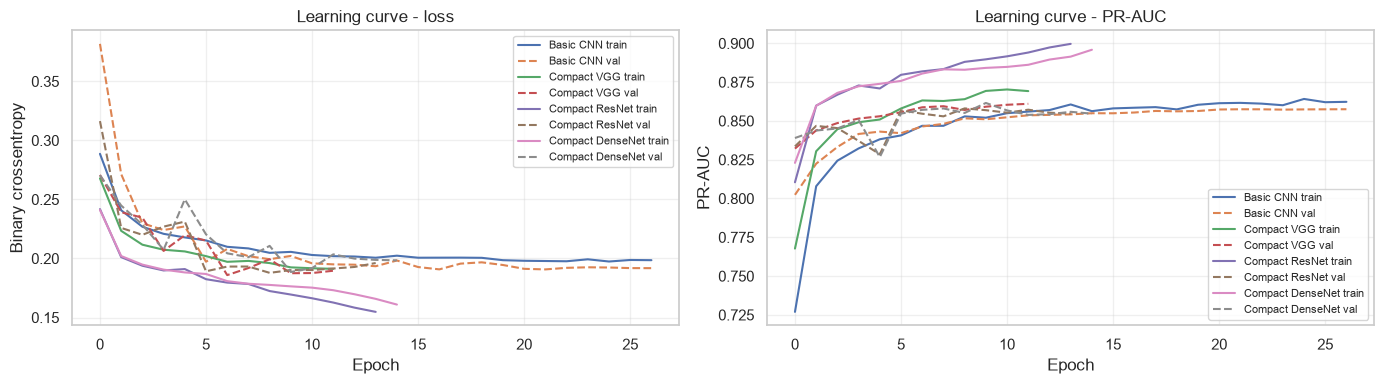
\includegraphics[width=\textwidth]{diabetes_learning_curves.png}
    \caption{Learning curves của bốn mô hình trên Diabetes}
    \label{fig:diabetes_learning_curves}
\end{figure}

Các mô hình đều hội tụ trong giới hạn 30 epoch.
Basic CNN chạy nhanh nhất nhưng có F1 thấp hơn nhóm kiến trúc sâu.
Compact DenseNet và Compact ResNet cho PR-AUC gần tương đương, cho thấy các kết nối tắt hoặc nối feature đều hữu ích khi mô hình sâu hơn baseline.

\section{Kết quả benchmark}
\begin{table}[H]
\centering
\caption{Benchmark bốn mô hình Conv1D trên Diabetes}
\label{tab:diabetes_benchmark}
\resizebox{\textwidth}{!}{%
\begin{tabular}{lcccccccccc}
\toprule
\textbf{Mô hình} & \textbf{Acc} & \textbf{Bal Acc} & \textbf{Precision} & \textbf{Recall} & \textbf{Spec} & \textbf{F1} & \textbf{ROC-AUC} & \textbf{PR-AUC} & \textbf{Threshold} & \textbf{Params} \\
\midrule
Compact ResNet & \best{0.9694} & 0.8575 & \best{0.9125} & 0.7217 & \best{0.9933} & \best{0.8060} & 0.9766 & 0.8840 & 0.865 & 242,273 \\
Compact DenseNet & 0.9686 & \best{0.8635} & 0.8889 & 0.7358 & 0.9911 & 0.8052 & 0.9767 & \best{0.8841} & 0.830 & 94,629 \\
Compact VGG & 0.9685 & 0.8570 & 0.9009 & 0.7217 & 0.9923 & 0.8014 & \best{0.9769} & 0.8804 & 0.815 & 159,265 \\
Basic CNN & 0.9651 & 0.8630 & 0.8453 & \best{0.7390} & 0.9869 & 0.7886 & 0.9766 & 0.8793 & 0.755 & 40,033 \\
\bottomrule
\end{tabular}%
}
\end{table}

\begin{figure}[H]
    \centering
    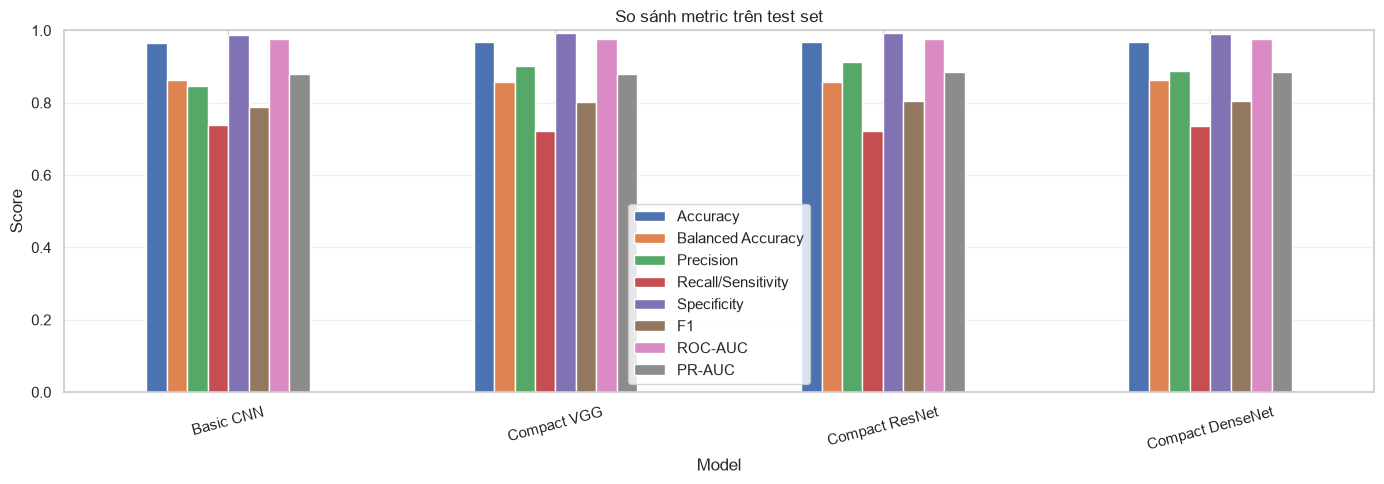
\includegraphics[width=\textwidth]{diabetes_metric_comparison.png}
    \caption{So sánh metric test của bốn mô hình trên Diabetes}
    \label{fig:diabetes_metric_comparison}
\end{figure}

\section{Ma trận nhầm lẫn và phân tích lỗi}
\begin{figure}[H]
    \centering
    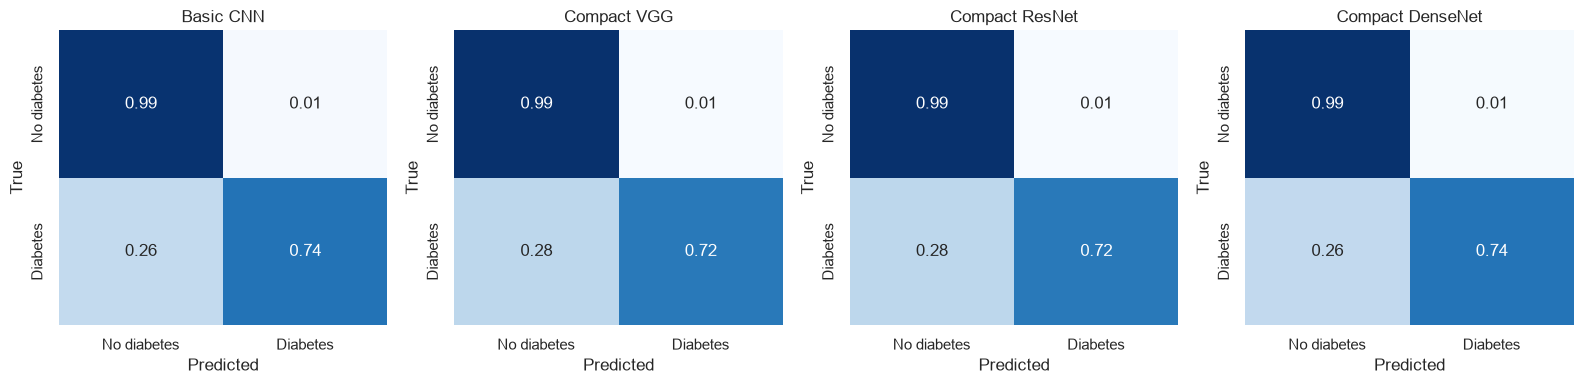
\includegraphics[width=\textwidth]{diabetes_confusion_matrices.png}
    \caption{Ma trận nhầm lẫn chuẩn hóa của bốn mô hình trên Diabetes}
    \label{fig:diabetes_confusion}
\end{figure}

Compact ResNet đạt F1 cao nhất 0.8060 với threshold 0.865.
Compact DenseNet đạt balanced accuracy và PR-AUC cao nhất rất sát ResNet.
Basic CNN có recall cao nhất nhưng specificity và precision thấp hơn, nghĩa là mô hình bắt được nhiều ca dương hơn nhưng tạo nhiều false positive hơn.
Với ứng dụng y tế, lựa chọn threshold cần phụ thuộc chi phí bỏ sót bệnh so với chi phí cảnh báo sai.

% =========================================================================
% CHUONG 5
% =========================================================================
\chapter{Thực Nghiệm Trên Fashion-MNIST}

\section{Khảo sát dữ liệu}
Fashion-MNIST gồm 60,000 ảnh train và 10,000 ảnh test, kích thước $28\times28\times1$.
Notebook tách 54,000 ảnh train và 6,000 ảnh validation bằng stratified split.
Các lớp gồm áo, quần, giày, túi và các nhóm trang phục có hình dạng gần nhau.

\begin{figure}[H]
    \centering
    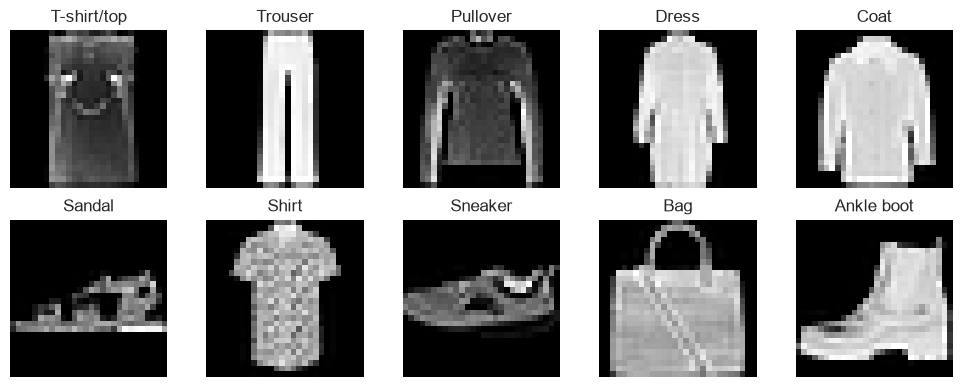
\includegraphics[width=0.95\textwidth]{fashion_sample_images.png}
    \caption{Ảnh mẫu của 10 lớp Fashion-MNIST}
    \label{fig:fashion_samples}
\end{figure}

\section{Tiền xử lý và cấu hình}
Ảnh được rescale về $[0,1]$ và chuẩn hóa bằng mean/std train.
Augmentation gồm horizontal flip, translation, rotation nhẹ và zoom.
Bốn kiến trúc Conv2D huấn luyện từ đầu, không dùng pretrained.
Tập test 10,000 ảnh chỉ được dùng sau khi đã chọn best weights bằng validation loss.

\section{Diễn biến huấn luyện}
\begin{figure}[H]
    \centering
    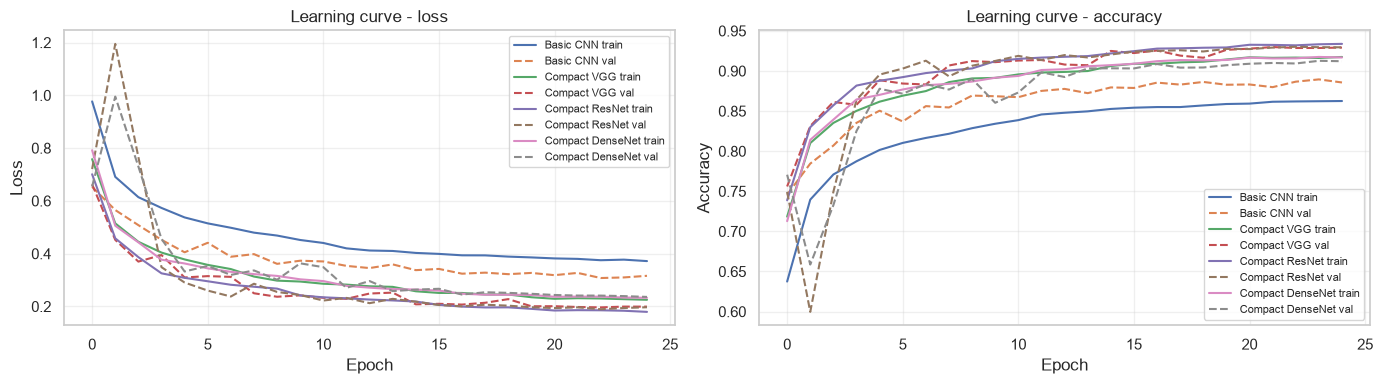
\includegraphics[width=\textwidth]{fashion_learning_curves.png}
    \caption{Learning curves của bốn mô hình trên Fashion-MNIST}
    \label{fig:fashion_learning_curves}
\end{figure}

Fashion-MNIST cân bằng giữa các lớp nên Accuracy và Macro F1 gần nhau.
Basic CNN học được baseline tốt nhưng kém nhóm mô hình sâu.
VGG cải thiện nhờ nhiều convolution $3\times3$.
ResNet đạt kết quả tốt nhất, cho thấy residual connection giúp mô hình sâu hơn ổn định trong cấu hình compact.

\section{Kết quả benchmark}
\begin{table}[H]
\centering
\caption{Benchmark bốn mô hình Conv2D trên Fashion-MNIST}
\label{tab:fashion_benchmark}
\resizebox{\textwidth}{!}{%
\begin{tabular}{lccccccccc}
\toprule
\textbf{Mô hình} & \textbf{Accuracy} & \textbf{Macro-P} & \textbf{Macro-R} & \textbf{Macro-F1} & \textbf{Loss} & \textbf{Params} & \textbf{Epoch tốt} & \textbf{Train(s)} & \textbf{Infer(s)} \\
\midrule
Compact ResNet & \best{0.9204} & \best{0.9201} & \best{0.9204} & \best{0.9199} & \best{0.2203} & 698,282 & 23 & 2,114.66 & 3.92 \\
Compact VGG & 0.9173 & 0.9190 & 0.9173 & 0.9178 & 0.2204 & 453,546 & 23 & 1,047.41 & 1.92 \\
Compact DenseNet & 0.9032 & 0.9031 & 0.9032 & 0.9030 & 0.2571 & 163,458 & 25 & 3,043.95 & 4.56 \\
Basic CNN & 0.8743 & 0.8766 & 0.8743 & 0.8746 & 0.3453 & 111,146 & 23 & \best{368.83} & \best{0.67} \\
\bottomrule
\end{tabular}%
}
\end{table}

\begin{figure}[H]
    \centering
    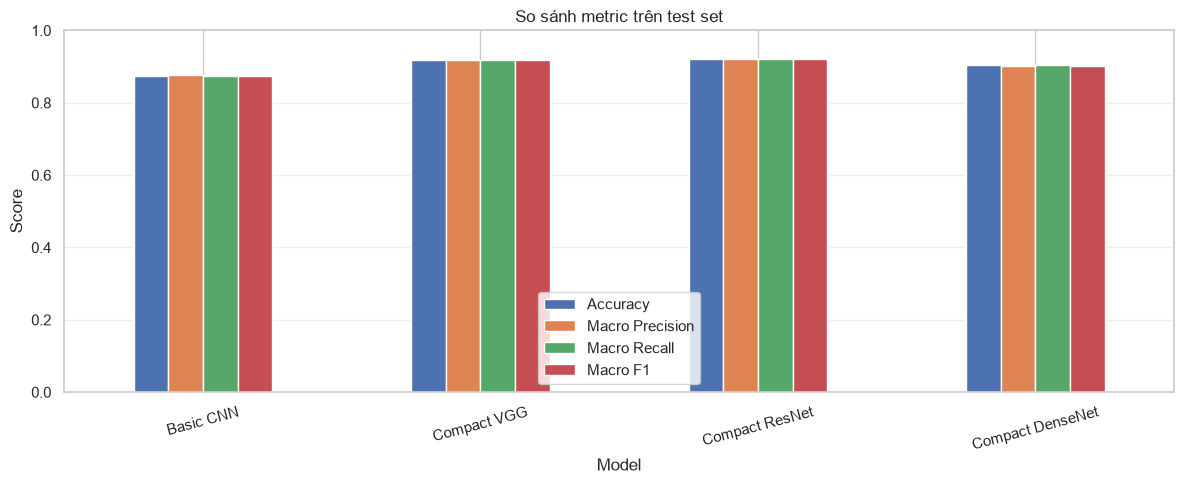
\includegraphics[width=\textwidth]{fashion_metric_comparison.png}
    \caption{So sánh metric test của bốn mô hình trên Fashion-MNIST}
    \label{fig:fashion_metric_comparison}
\end{figure}

\section{Ma trận nhầm lẫn và phân tích lỗi}
\begin{figure}[H]
    \centering
    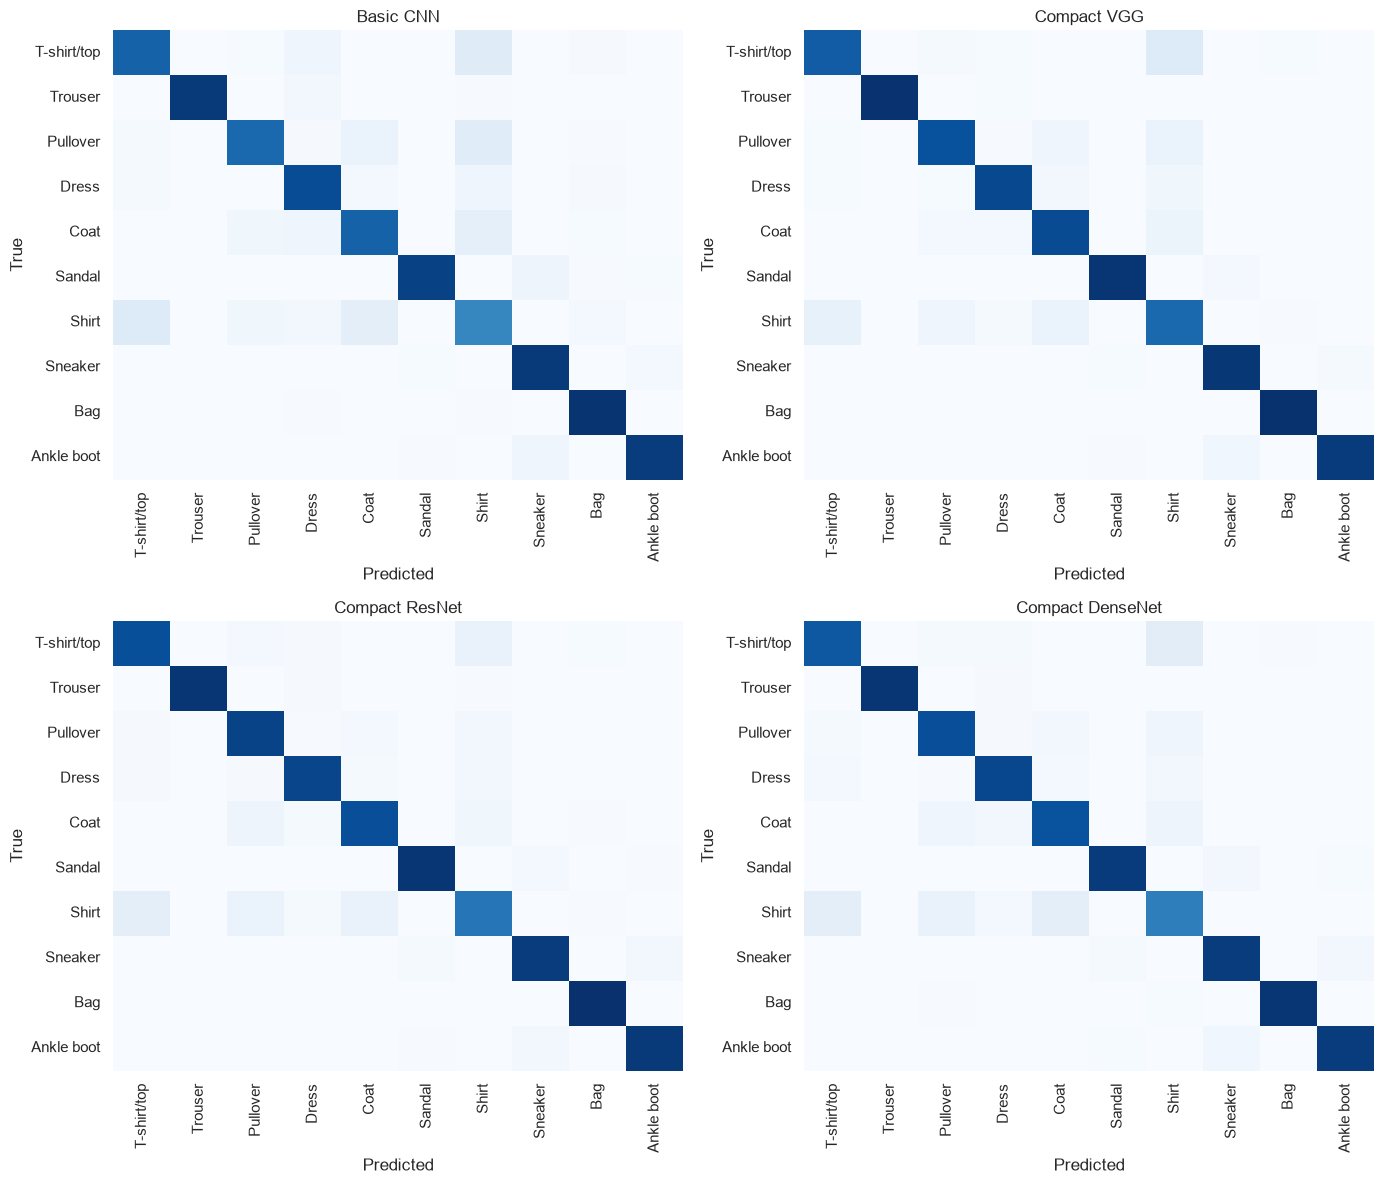
\includegraphics[width=\textwidth]{fashion_confusion_matrices.png}
    \caption{Ma trận nhầm lẫn chuẩn hóa của bốn mô hình trên Fashion-MNIST}
    \label{fig:fashion_confusion}
\end{figure}

Compact ResNet đạt Macro F1 cao nhất 0.9199 và accuracy 0.9204.
Compact VGG đứng rất gần với Macro F1 0.9178, trong khi DenseNet thấp hơn dù có ít tham số hơn VGG và ResNet.
Những nhầm lẫn phổ biến thường xuất hiện giữa shirt, pullover và coat vì các lớp này có silhouette tương tự ở ảnh xám độ phân giải thấp.

\begin{figure}[H]
    \centering
    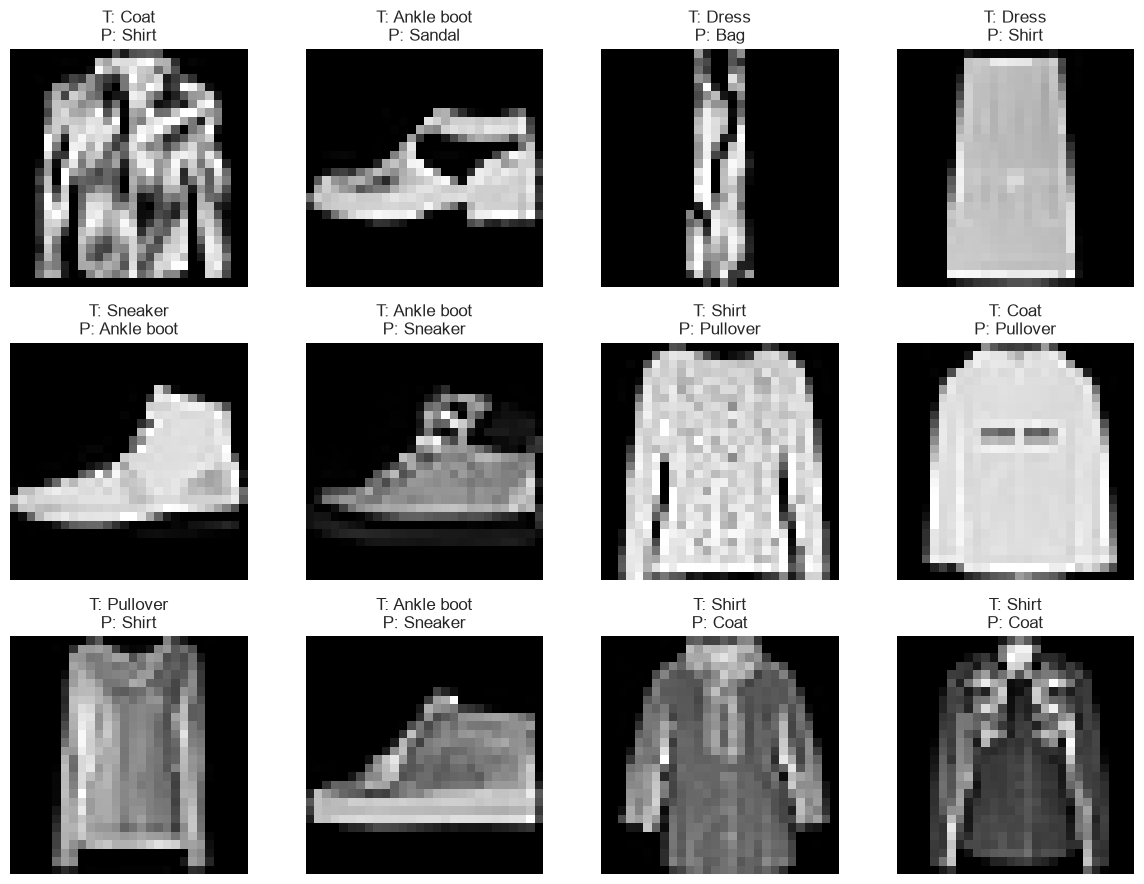
\includegraphics[width=0.88\textwidth]{fashion_prediction_error_analysis.png}
    \caption{Một số dự đoán sai của mô hình tốt nhất trên Fashion-MNIST}
    \label{fig:fashion_errors}
\end{figure}

% =========================================================================
% CHUONG 6
% =========================================================================
\chapter{Thực Nghiệm Trên CIFAR-100}

\section{Khảo sát dữ liệu}
CIFAR-100 gồm 50,000 ảnh train và 10,000 ảnh test, ảnh màu $32\times32\times3$.
Bộ dữ liệu có 100 lớp fine-grained, mỗi lớp có 500 ảnh train gốc và 100 ảnh test.
Notebook tách 45,000 ảnh train và 5,000 ảnh validation bằng stratified split.

\begin{figure}[H]
    \centering
    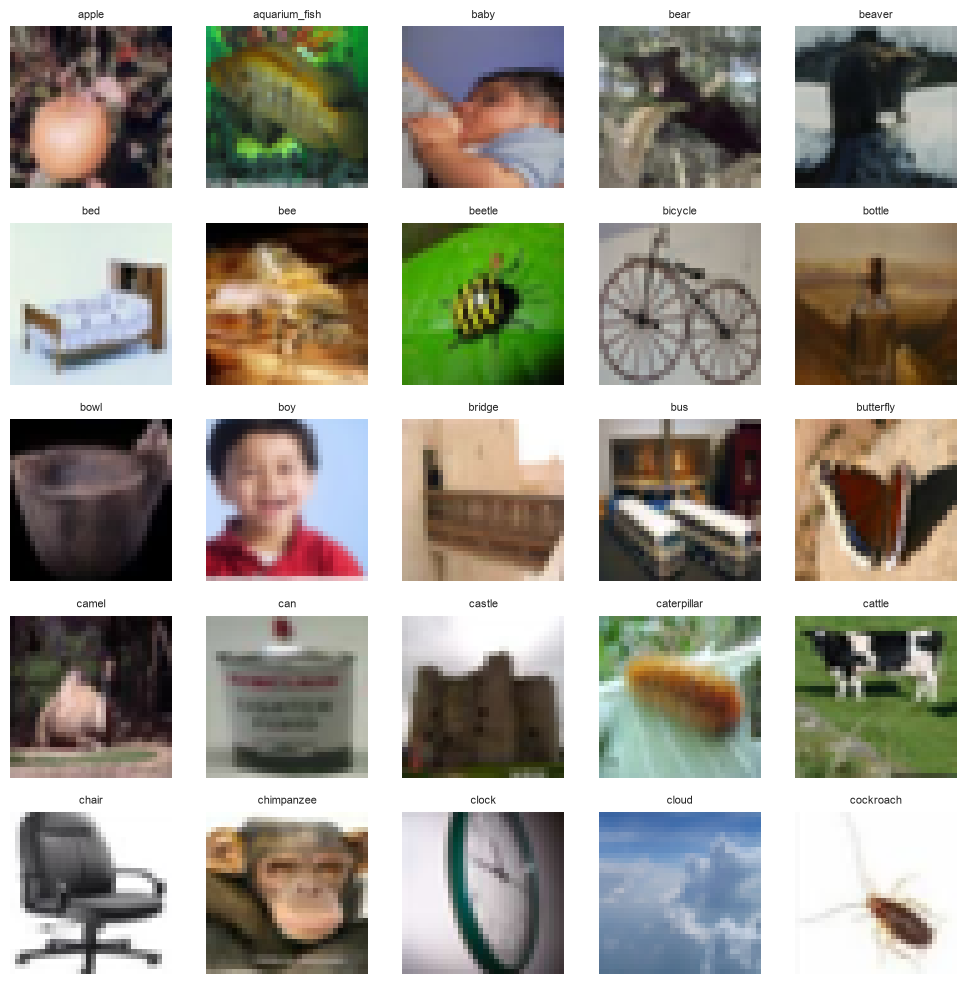
\includegraphics[width=0.90\textwidth]{cifar100_sample_images.png}
    \caption{Ảnh mẫu của một số lớp đầu tiên trong CIFAR-100}
    \label{fig:cifar100_samples}
\end{figure}

\section{Tiền xử lý và cấu hình}
Archive \modelpath{cifar-100-python.tar.gz} được tải từ nguồn chính thức và kiểm tra MD5.
Notebook đọc các file pickle \modelpath{train}, \modelpath{test} và \modelpath{meta}.
Ảnh được reshape về $(N,32,32,3)$.
Augmentation gồm horizontal flip, translation, rotation, zoom và contrast nhẹ.
Do số lớp lên tới 100, bài toán khó hơn đáng kể so với Fashion-MNIST.

\section{Diễn biến huấn luyện}
\begin{figure}[H]
    \centering
    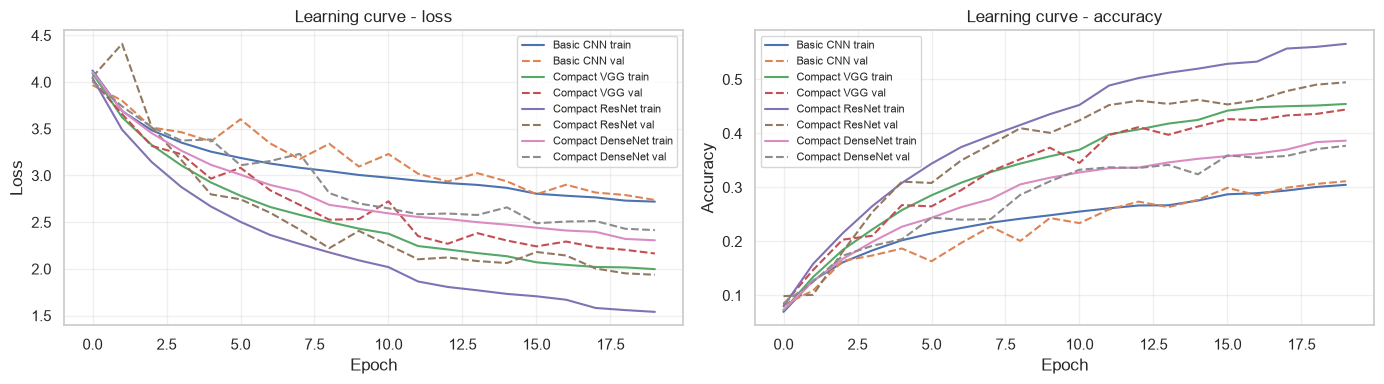
\includegraphics[width=\textwidth]{cifar100_learning_curves.png}
    \caption{Learning curves của bốn mô hình trên CIFAR-100}
    \label{fig:cifar100_learning_curves}
\end{figure}

Trong giới hạn 20 epoch, tất cả mô hình đều có best epoch bằng 20.
Điều này cho thấy mô hình vẫn còn khả năng cải thiện nếu tăng số epoch hoặc dùng lịch learning rate dài hơn.
Dù vậy, benchmark vẫn đủ để so sánh xu hướng: ResNet tốt nhất, VGG đứng thứ hai, DenseNet và Basic CNN thấp hơn.

\section{Kết quả benchmark}
\begin{table}[H]
\centering
\caption{Benchmark bốn mô hình Conv2D trên CIFAR-100}
\label{tab:cifar100_benchmark}
\resizebox{\textwidth}{!}{%
\begin{tabular}{lccccccccc}
\toprule
\textbf{Mô hình} & \textbf{Accuracy} & \textbf{Macro-P} & \textbf{Macro-R} & \textbf{Macro-F1} & \textbf{Loss} & \textbf{Params} & \textbf{Epoch tốt} & \textbf{Train(s)} & \textbf{Infer(s)} \\
\midrule
Compact ResNet & \best{0.5062} & \best{0.5665} & \best{0.5062} & \best{0.5055} & \best{1.8785} & 710,468 & 20 & 2,018.57 & 6.70 \\
Compact VGG & 0.4501 & 0.5011 & 0.4501 & 0.4447 & 2.1184 & 465,732 & 20 & 988.18 & 2.58 \\
Compact DenseNet & 0.3796 & 0.4288 & 0.3796 & 0.3719 & 2.3846 & 174,564 & 20 & 2,841.07 & 6.74 \\
Basic CNN & 0.3156 & 0.3639 & 0.3156 & 0.3035 & 2.7271 & 123,332 & 20 & \best{373.66} & \best{0.97} \\
\bottomrule
\end{tabular}%
}
\end{table}

\begin{figure}[H]
    \centering
    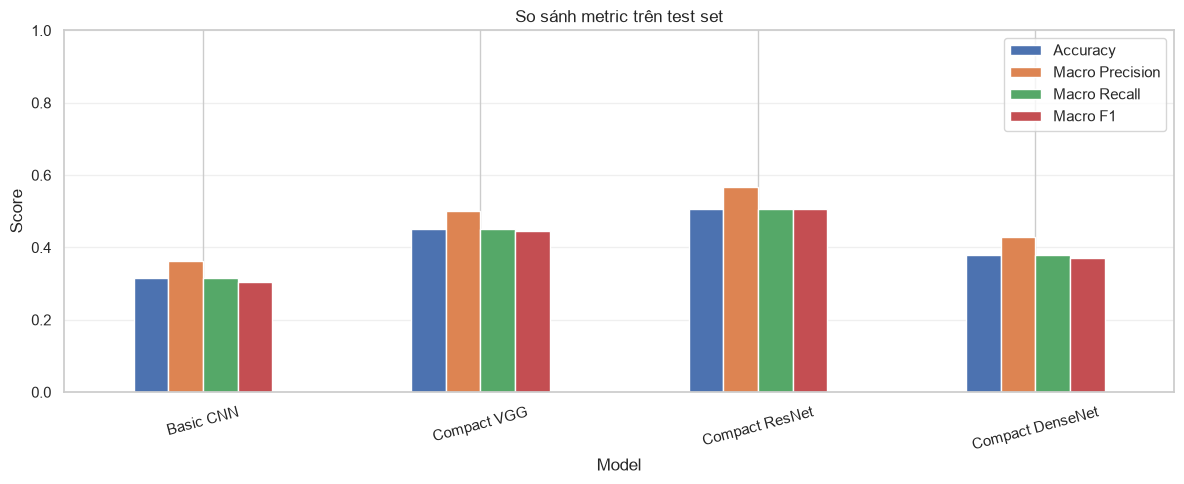
\includegraphics[width=\textwidth]{cifar100_metric_comparison.png}
    \caption{So sánh metric test của bốn mô hình trên CIFAR-100}
    \label{fig:cifar100_metric_comparison}
\end{figure}

\section{Ma trận nhầm lẫn và phân tích lỗi}
\begin{figure}[H]
    \centering
    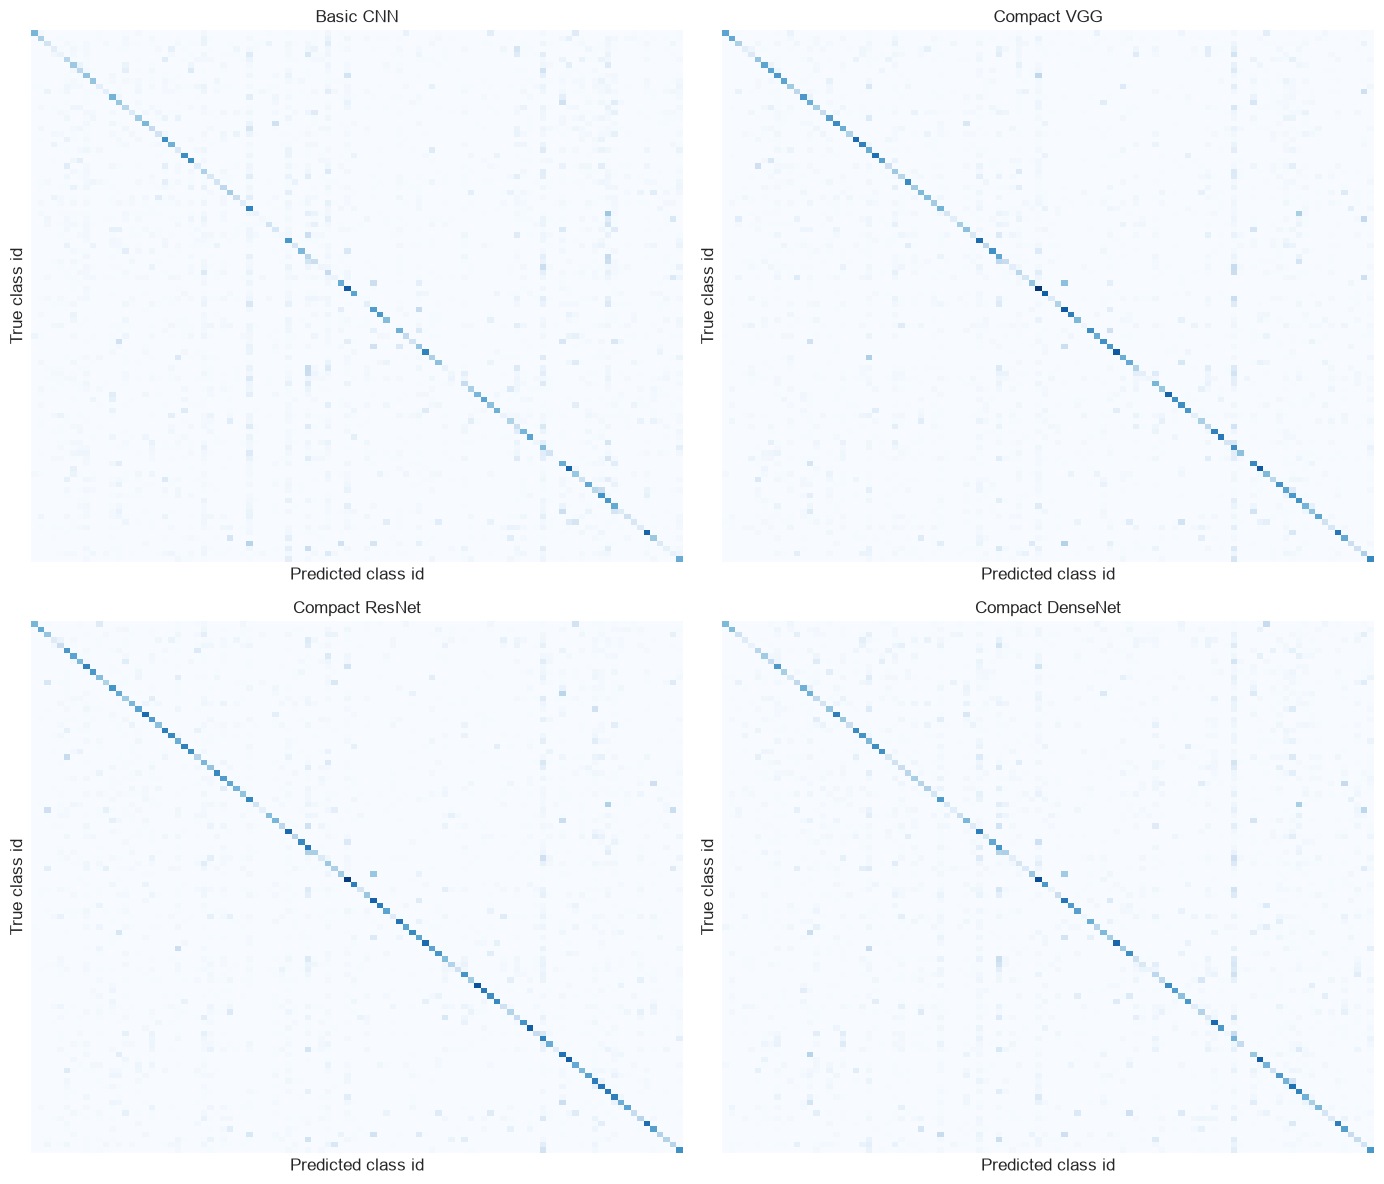
\includegraphics[width=\textwidth]{cifar100_confusion_matrices.png}
    \caption{Ma trận nhầm lẫn chuẩn hóa của bốn mô hình trên CIFAR-100}
    \label{fig:cifar100_confusion}
\end{figure}

Compact ResNet đạt Macro F1 0.5055 và accuracy 0.5062, cao nhất trong bốn mô hình.
Khoảng cách giữa ResNet và Basic CNN hơn 20 điểm phần trăm accuracy, cho thấy dữ liệu nhiều lớp cần kiến trúc có khả năng truyền gradient tốt.
Tuy nhiên, CIFAR-100 vẫn còn khó trong cấu hình compact 20 epoch; nhiều lớp có hình dạng hoặc ngữ nghĩa gần nhau dễ bị nhầm.

\begin{figure}[H]
    \centering
    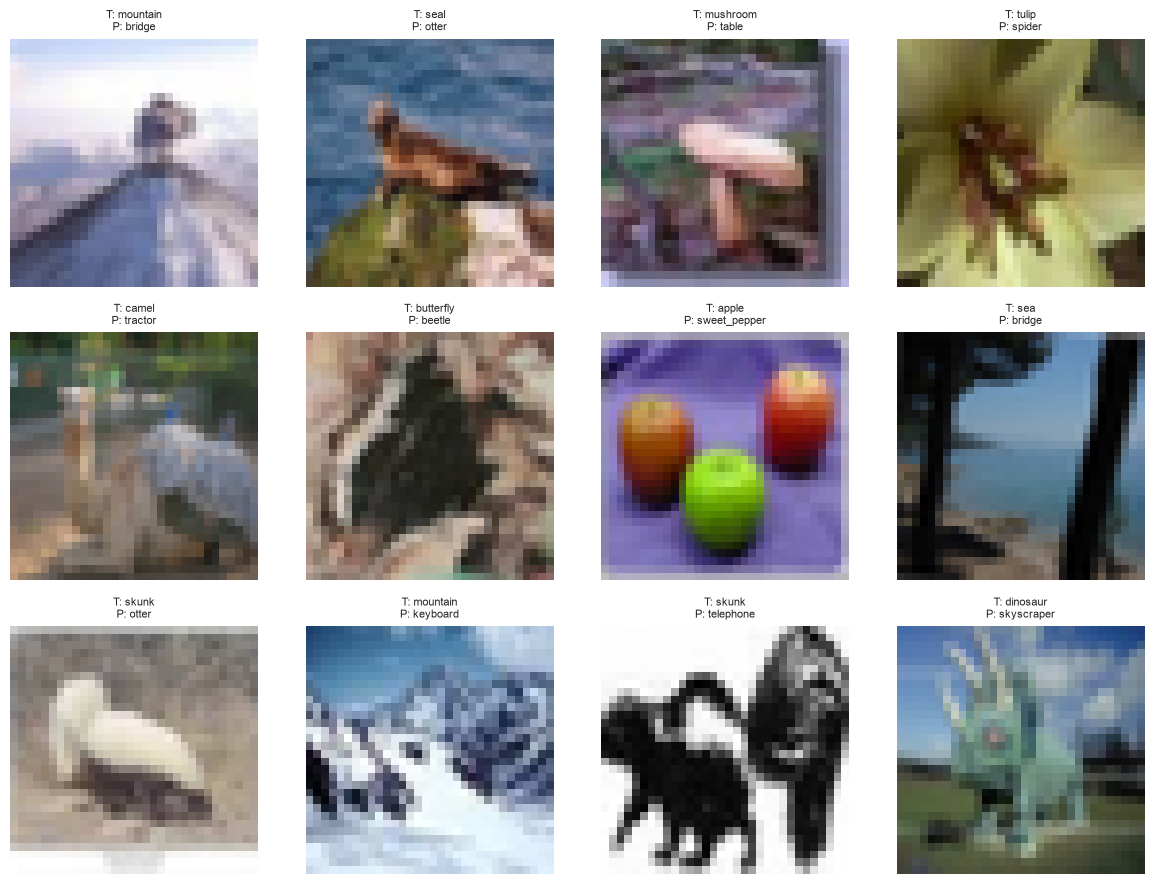
\includegraphics[width=0.88\textwidth]{cifar100_prediction_error_analysis.png}
    \caption{Một số dự đoán sai của mô hình tốt nhất trên CIFAR-100}
    \label{fig:cifar100_errors}
\end{figure}

% =========================================================================
% CHUONG 7
% =========================================================================
\chapter{Tổng Hợp Đối Chuẩn Và Kết Luận}

\section{Tổng hợp kết quả chính}
\begin{table}[H]
\centering
\caption{Mô hình tốt nhất theo metric chính của từng dataset}
\label{tab:master_summary}
\resizebox{\textwidth}{!}{%
\begin{tabular}{llccccc}
\toprule
\textbf{Dataset} & \textbf{Mô hình tốt nhất} & \textbf{Metric chính} & \textbf{Score} & \textbf{Accuracy} & \textbf{Params} & \textbf{Train(s)} \\
\midrule
Diabetes & Compact ResNet & F1 & \best{0.8060} & 0.9694 & 242,273 & 78.77 \\
Fashion-MNIST & Compact ResNet & Macro-F1 & \best{0.9199} & 0.9204 & 698,282 & 2,114.66 \\
CIFAR-100 & Compact ResNet & Macro-F1 & \best{0.5055} & 0.5062 & 710,468 & 2,018.57 \\
\bottomrule
\end{tabular}%
}
\end{table}

Trong cả ba dataset, Compact ResNet là mô hình có metric chính cao nhất.
Kết quả này phù hợp với trực giác lý thuyết: residual connection giúp mô hình sâu hơn vẫn tối ưu ổn định.
VGG cũng mạnh trên ảnh, đặc biệt Fashion-MNIST, nhưng thiếu shortcut nên khó vượt ResNet trong cùng số epoch.
DenseNet có số tham số thấp hơn ResNet ở cả ba dataset, nhưng trong các lần chạy này chưa đạt score cao nhất.

\section{So sánh theo độ khó dữ liệu}
Diabetes có accuracy cao vì lớp âm chiếm đa số, nhưng F1 chỉ quanh 0.80 do bài toán mất cân bằng.
Fashion-MNIST cân bằng và có 10 lớp, ảnh đơn giản hơn CIFAR-100 nên Compact ResNet đạt Macro F1 0.9199.
CIFAR-100 có 100 lớp và chỉ 500 ảnh train gốc mỗi lớp, vì vậy Macro F1 0.5055 trong 20 epoch phản ánh độ khó fine-grained classification.

\section{Công bằng và giới hạn của benchmark}
Benchmark giữ cùng split, preprocessing, optimizer và callback trong từng dataset.
Tuy nhiên, thời gian train phụ thuộc trạng thái máy và backend TensorFlow tại thời điểm chạy.
Số epoch CIFAR-100 bị giới hạn ở 20 để phù hợp thời gian CPU, nên kết quả chưa đại diện cho khả năng tối đa của từng kiến trúc.
Ngoài ra, Conv1D trên Diabetes chỉ là minh họa kiến trúc CNN trên dữ liệu bảng; để tối ưu bài toán thực tế cần so sánh thêm với mô hình chuyên cho tabular.

\section{Kiểm toán khả năng tái lập}
\begin{table}[H]
\centering
\caption{Checklist tái lập Assignment 05}
\label{tab:reproducibility}
\resizebox{\textwidth}{!}{%
\begin{tabular}{lll}
\toprule
\textbf{Hạng mục} & \textbf{Cách thực hiện} & \textbf{Ý nghĩa} \\
\midrule
Random seed & Seed 42 cho NumPy, Python và TensorFlow & Giảm dao động split và khởi tạo \\
Split dữ liệu & Stratified train/validation/test & Giữ phân phối lớp ổn định \\
Preprocessing & Fit scaler hoặc mean/std chỉ trên train & Chống data leakage \\
Augmentation & Chỉ hoạt động trong training & Validation/test phản ánh dữ liệu gốc \\
Callback & ReduceLROnPlateau và EarlyStopping & Ổn định huấn luyện \\
Threshold Diabetes & Chọn trên validation, khóa khi test & Không chọn threshold từ test \\
Metric & Accuracy, macro metric, F1, AUC và thời gian & So sánh chất lượng và chi phí \\
\bottomrule
\end{tabular}%
}
\end{table}

\section{Kết luận}
Báo cáo đã xây dựng và đối chuẩn bốn kiến trúc CNN compact trên ba dataset của Assignment 05.
Các kết luận chính gồm:
\begin{enumerate}
    \item CNN có thể được hiểu thống nhất dưới dạng hàm hợp từ convolution, BatchNorm, ReLU, pooling đến classifier.
    \item VGG tăng năng lực biểu diễn bằng cách chồng nhiều convolution $3\times3$.
    \item ResNet đạt kết quả tốt nhất trên cả Diabetes, Fashion-MNIST và CIFAR-100 nhờ residual connection.
    \item DenseNet có lợi thế tái sử dụng feature và số tham số thấp hơn ResNet, nhưng chưa thắng trong các cấu hình compact đã chạy.
    \item Độ khó dữ liệu tăng rõ từ Fashion-MNIST sang CIFAR-100, thể hiện qua Macro F1 giảm từ 0.9199 xuống 0.5055.
\end{enumerate}

Hướng mở rộng gồm chạy nhiều seed để báo cáo độ ổn định, tăng epoch cho CIFAR-100, thử lịch cosine decay, mixup/cutout và so sánh thêm với mô hình tabular chuyên dụng cho Diabetes.

\end{document}
